
\section{Implementation and Evaluation}

\subsection{Turing Machine}

% Target_fn returning next step given access to current state in global vars
%   - busy beaver
%   - cache page speculation on repetetive cycles. 
%       - mis-predict w/in speculative world 

% speed (complete smaller busy beaver?)
% against reference python implementation?

\subsection{AES Decryption}

% implementation 
%   Key Schedule expansion / obfuscation
%
% you can speculatively execute AES instructions 

\subsection{Virtual Machine}


\subsubsection{SPASM}
\label{subsubsec:spasm}
Constructing an emulator making use of the speculative primitive requires  
a trade off in expresive capability versus speed. 
We have implemented SPASM as a model using two pseudo-registers, and six 
bit instruction length which allows for a relatively direct programming model 
in which structured values can be entered into memory locations before making 
a systemcall.

To acheive a balance with speed the number of bits in each instruction is both 
fixed and minimized.  A variable length instruction would require that the prime
and probe stage search the maximum number of bits on each round, and each 
aditional bit doubles the search space that the prime and probe stage must 
traverse.  So every bit shorted effectively doubles the throughput of the 
emulator, and there is effectively no advantage to allowing variable length 
instructions. 

Using this model we have implemented multiple example programs that can be run
as encrypted payloads in an \speculake payload. A \textit{HelloWorld} program 
that prints to stdout. A \textit{FizzBuzz} program that demonstrates control 
flow and arithmetic operations while printing to stdout. And finally,
a \textit{ReverseShell} program that opens and connects to a socket before  
duplicating I/O and executing a local shell. 

Expected performance for a given SPASM binary will vary given multiple factors, 
the most important of which is the prime and probe redundancy. This can be tuned
based on the specific trigger, as it is used to establish confidence that a signal 
has been identified in the indicess returned from the "speculative world". 
Thus accomplishing a task using SPASM generally equates to:

\begin{lstlisting}
    Redundancy * Probe_Space * Num_Instr
\end{lstlisting}

For example, the \textit{ReverseShell} program makes six system calls to open a socket,
connect to it, duplicate I/O, and execve a specified program. This requires 355
SPASM instructions to complete. The probe space for the 6-bit SPASM ISA requires 
a traversal of an array od size 64. When using a redundancy of 256 to establish
confidence in the signal the entire \textit{ReverseShell} program takes under 7 
seconds to run once triggered. 

\begin{figure}[b]
    \centering
        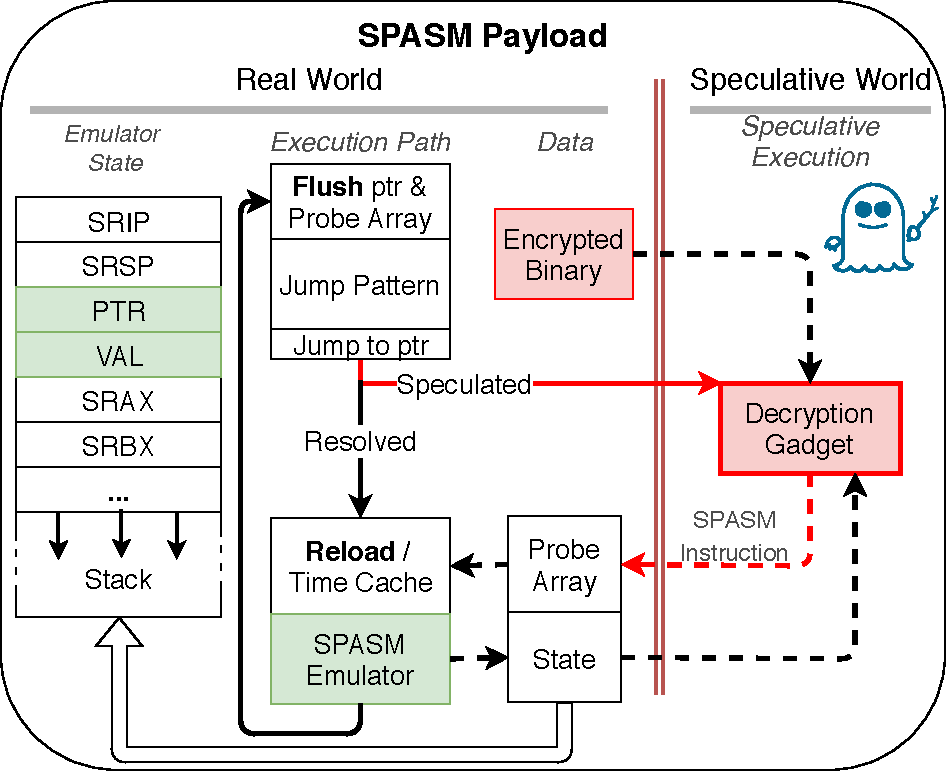
\includegraphics[width=0.5\textwidth]{figures/spasm_model}
    \caption{This model describes the VM control flow. An encrypted SPASM binary 
        stored in dead code or data accessible to \textit{Speculative Computation} 
        is decrypted  and then returned through the primitive. The SPASM 
        \textit{Resultant Computation} performs the SPASM emulation to update the 
        process state before the next instruction is decrypted.}
    \label{fig:spasm_model}
\end{figure}

\subsubsection{ARM}
\label{subsubsec:arm}
While the custom emulator that we developed gives a much higher level abstraction to 
a developer, it still requires programs to be written in custom assembly 
language. To demonstrate that the extensibility of this model we also implemeted a wrapper
around an ARM emulator, such that programs can be written in a high level languages 
such as C or C++, statically compiled to binaries for the ARM emulator, and deployed 
as an encrypted data sections to be decrypted at run-time.  


% ARM Wrapper
%   - memory
%   - single instruction vs block

We chose to implement a wrapper around ARM as it has a 32-bit fixed instruction
length. However this causes a significant hit to the speed at which operations 
can be performed as the probe space is increased by a factor of four in 
comparison with SPASM,  and we must complete 4 of these transactions to 
retreive a single ARM opcode. Trading more expressive operations for speed
results in a 16x slowdown when considering per-instruction throughput. 

\begin{lstlisting}
    4 * Redundancy * Probe_Space * Num_Instr
\end{lstlisting}

\subsection{OpenSSL Trigger}

% extract jump patterns
% sufficiency checks 
%
% trigger strength
%   - future work developing tools to determine sufficiency and strength
%
% OPENSSL TRIGGERING REVERSE SHELL SPASM PAYLOAD

%%%%%%%%%%%%%%
